%        File: resumo.tex
%     Created: seg jul 29 09:00  2019 -0
% Last Change: seg jul 29 09:00  2019 -0
%
\documentclass[a4paper]{article}
\usepackage[brazilian]{babel}
\usepackage[utf8]{inputenc}
\usepackage[T1]{fontenc}
\usepackage{graphicx}
\usepackage{microtype}          % para melhorias de justificação
\usepackage{natbib}
\usepackage[bookmarks]{hyperref}



\graphicspath{ {./imagens/} }

\makeindex

\begin{document}

\section{Aula introdutória}
\subsection{Paralelismo}
involve paralelismo das intruções, tarefas e processos.
Sendo os dois primeiros envolvidos com o baixo nível(pipeline, multThread(hiperThread)) e o terceiro a quantidade de processadores.
\section{Desempenho}
\subsection{Introdução}
    Desempenho é medido em 1 sobre tempo de execução e a comparação é desempenho x sobre desempenho y
\subsection{Tempo de execução}
Tempo de resposta, tempo decorrido. Para arquitetura só conta o tempo da CPU, que é o tempo de usuário(modo usuário)
mais o tempo de sistema(modo kernel), o foco é o tempo de CPU de usuário.

\subsection{Ciclos de clock}
Ciclo de clock é a menor unidade de tempo da arquitetura.

Ele contém características como frequência e período(tempo de ciclo).Sendo que a primeira é consequencia da segunda.

Calculo do tempo: t =  ciclos * tempo de ciclo.

Para melhorar o tempo é necessário diminuir a quantidade de ciclos ou diminuir o tempo de ciclo, porém você pode
aumentar um e diminuir o outro, por exemplo multiciclo usa mais ciclos porém consegue diminuir o período de forma a
compensar o ganho em ciclos.

Para diminuir a quantidade de ciclos de um programa, poder ser alcançado com o uso do compilador ou com a melhoria do
programa.

Não podemos considerar que instruções tenham o mesmo tempo de execução que outra instrução, já que adição é mais rápido
que o acesso a memória.

Ciclos podem ser iguais a CPI * qtdDeInstruções

CPI = Clocks Per Instruction

IPC = Instructions Per Clock

IPC é o inverso do CPI e os seus valores mudam de acordo com a organização da CPU:

Monociclo:

    CPI = 1

    IPC = 1

Multiciclo:

    CPI = média dos ciclos usados pelas instruções

    IPC = 1/CPI


Pipeline:

    CPI = algo proximo de 1

    IPC = algo proximo de 1

\subsection{Exemplo}
A gente tem um programa e ele demora 10s para ser executado no computador A e que possui um clock de 4Ghz e queremos
construir uma máquina B e deve executar o programa em 6s porém o aumento do clock resultara em um aumento de 1.2 ciclos
a mais no programa.

t = ciclos * tempo de ciclo

10 = X * 250 * $10^{-12}$

X = $\frac{10^{13}}{250}$

X = $4 * 10^{10}$ qtd de Ciclos

Y = 1.2 * X

Y = 4.8 * $10^{10}$ qtd de Ciclos

Z Ghz = $\frac{1}{\frac{6}{Y}}$

Z Ghz = 8 Ghz

\subsection{LEi de Amdahl}
É uma formula para determinar quantas melhorias devem ser feitas para que uma operação diminua o custo do programa como
um todo.

Tempo final = Tempo não alterado + (tempo de execução afetado / quantidades de melhorias)

\subsection{Resumo}
Desempenho é o tempo de execução da aplicação, velocidade de uma maquina x em relação ao uma maquina y é $y/x$.

MIPS também Milhões de instruções por segundo.

\section{RISC}
RISC é um tipo e arquitetura de processador, cujas características são poucas intruções, poucos tipos de instruções,
poucos modos de endereçamento ,  load/store(só faz operações com dados nos registradores).
\section{ Pipeline }
\subsection{Introdução}
    O pipeline é a divisão da instrução em etapas de forma a tornar possível a sobreposição de execução de instruções.
    Dessa forma executando mais de ums intrução ao mesmo tempo.

    O pipeline é dividido em 5 etapas, não quer dizer que todas as intruções execute todas as etapas.
    \begin{itemize}
        \item \textbf{IF} Busca da instrução.
        \item \textbf{ID} Decodificação e busca dos operandos.
        \item \textbf{EX} Execução.
        \item \textbf{MEM} Acesso à memória de dados.
        \item \textbf{WB} Escrita de volta no Banco de registradores.
    \end{itemize}
\subsection{Nomenclatura}
    O que está sombreado é utilizado, a metade da direita é leitura a metade da esquerda é escrita, há também a mostra
    do que está sendo usado em cada estágio do pipeline.

    \begin{figure}
        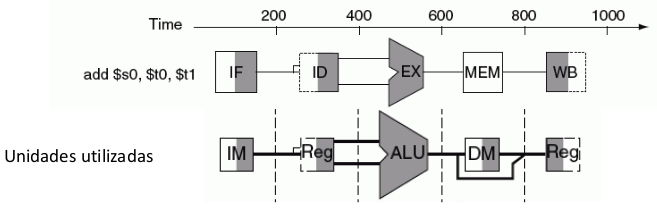
\includegraphics[width=1.2\textwidth]{nomenclatura}
    \end{figure}

\subsection{Implementação}

Armazenamento estável são os registradores, ou qualquer lugar onde os dados não se percam.

\begin{figure}[h]
        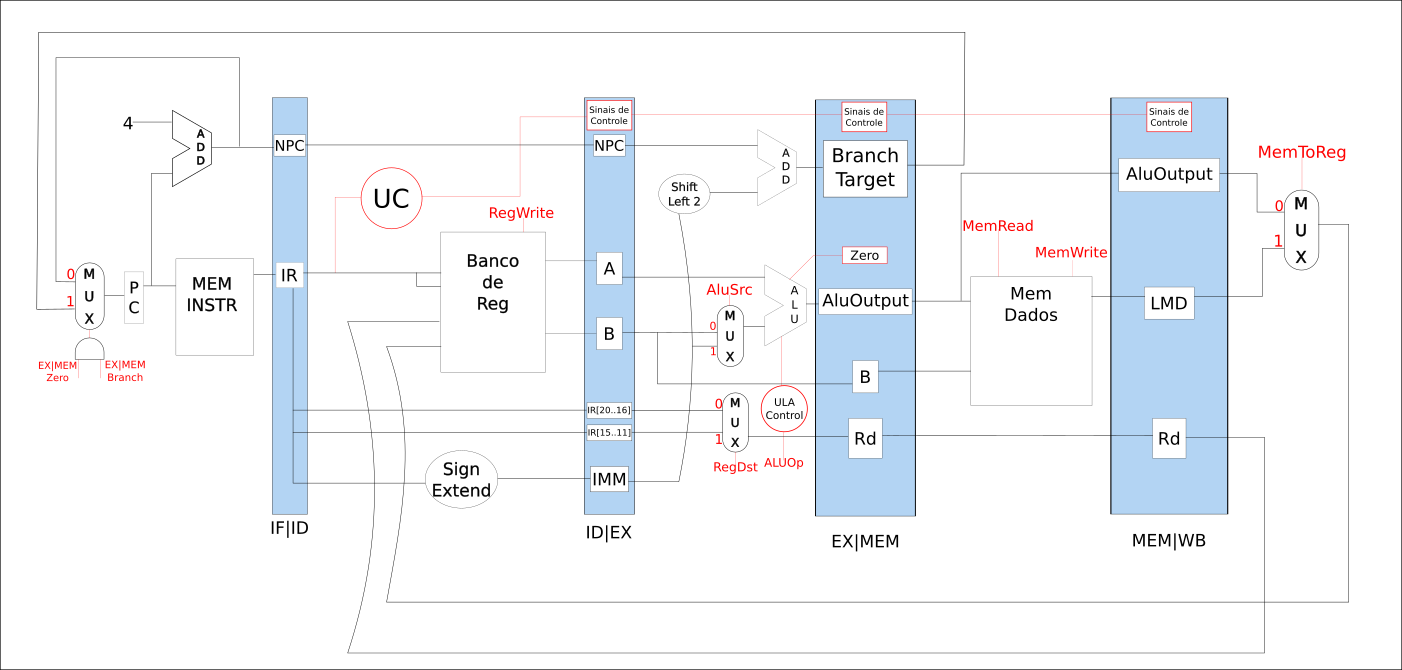
\includegraphics[width=13cm]{implementacao}
\end{figure}
% colocar o zero da ULA o estágio EX|MEM
\begin{itemize}
    \item IF|ID
        \begin{itemize}
            \item IF|ID.IR
            \item IF|ID.NPC
        \end{itemize}
    \item ID|EX
        \begin{itemize}
            \item ID|EX.NPC
            \item ID|EX.A
            \item ID|EX.B
            \item ID|EX.Imm
            \item ID|EX.IR[20..16]
            \item ID|EX.IR[15..11]
        \end{itemize}
    \item EX|MEM
        \begin{itemize}
            \item EX|MEM.AluOutput
            \item EX|MEM.B
            \item EX|MEM.BranchTarget
            \item EX|MEM.Rd
        \end{itemize}
    \item MEM|WB
        \begin{itemize}
            \item MEM|WB.LMD
            \item MEM|WB.AluOutput
            \item MEM|WB.Rd
        \end{itemize}
\end{itemize}

Esses são registradores para que cada fase do pipeline consiga executar a instrução corretamente.
Por isso o NPC é feito em duas fases diferentes pois o valor dele é utlizado somente na fase de execução do Branch.

O estágio de WB necessita do IR para saber o endereço do registrador que vai receber os dados, então por isso é puxado
mais dois campos no estágio ID|EX para poder salvar os possíveis endereços de registrador para salvar os dados no
estágio WB. Porém somente no estágio EX que os sinais de controles estão prontos, então nesse estágio é decidido qual
dos dois endereços vai ser usado para salvar o dado.

\subsection{Unidade de controle}
A unidade de controle vai ter os seus sinais salvos na fase ID/EX e os que não forem usados vai ser salvo nos estágios
seguintes, IF e ID não tem sinal de controle.Segue os sinais de controle.

\begin{itemize}
    \item EX
        \begin{itemize}
            \item AluOp
            \item AluSrc
            \item RegDst
        \end{itemize}
    \item MEM
        \begin{itemize}
            \item MemRead
            \item MemWrite
        \end{itemize}
    \item WB
        \begin{itemize}
            \item MemToReg
            \item RegWrite
            \item branch
        \end{itemize}
\end{itemize}

Esses sinais vão ser armazenados nos estágios ID|EX , EX|MEM , MEM|WB. Quando o processador para de armazenar os sinais
quando ele chega no estágio em que ele é utilizado.

Segue  a lista de registradores em cada estágio:
\begin{itemize}
    \item IF|ID
        \begin{itemize}
            \item NPC
            \item IR
        \end{itemize}
    \item ID|EX
        \begin{itemize}
            \item NPC
            \item A
            \item B
            \item Imm
            \item IR[20..16]
            \item IR[15..11]
            \item AluSrc
            \item AluOp
            \item RegDst
            \item MemRead
            \item MemWrite
            \item Branch
            \item MemToReg
            \item RegWrite
        \end{itemize}
    \item EX|MEM
        \begin{itemize}
            \item BranchTarget
            \item AluOutput
            \item Rd
            \item B
            \item MemRead
            \item MemWrite
            \item Branch
            \item zero
            \item MemToReg
            \item RegWrite
        \end{itemize}
    \item MEM|WB
        \begin{itemize}
            \item LMD
            \item AluOutput
            \item Rd
            \item MemToReg
            \item RegWrite
        \end{itemize}
\end{itemize}


\section{Dependências do Pipeline}
\subsection{Introdução}
    Problema que faz com que o pipeline pare por um tempo.
    Isso pode ocorrer em tres casos diferentes:
    \begin{itemize}
        \item Acesso concorrente a mesma estrutura.
        \item Utilização de um dado ainda não ``finalizado''.
        \item Busca e execução de instrução erradas(Branch).
    \end{itemize}

\subsection{Dependencia Estrutural}
    É quando duas instruçoes precisam executar em uma mesma estrutura. por exemplo a beq precisa utilizar a ULA duas
    vezes, quando calcular o novo endereço e para fazer a compração, o MIPS resolve isso duplicando as estruturas,
    quando é possível.

\subsection{Dependência de dados}
    É quando uma instrução por exemplo uma add que salva o resultado no registrador \$t0 e a proxima instrução vai
    utilizar o resultado dessa soma, só que o resultado da soma ainda não está no \$t0.

    \subsubsection{Dependências Verdadeitas}
    Também chamado de RAW (Read After Write),É o caso do exemplo dado acima. Dependências verdadeiras que param o
    pipeline são chamadas de \textit{Hazard} quando elas realmente atrapalham a execução, ou seja tem que ter menos de 1 instrução entre elas .


    \subsubsection{Dependência Falsas}

    Dependencia falsa acontece quando se usa técnicas de execução fora de ordem.

    \textbf{Antidependência} também chamda de WAR(write after read).
    dado o seguinte código:

    sub \$t4 \$t0 \$t5
    add \$t0 \$t1 \$t2

    Esse código não tem problema, porém se a arquitetura utilizar exeução fora de ordem pois ele pode tentar fazer o add
    antes da sub.

    \textbf{Dependência de Saida}
    Também chamada de WAW( Write After Write).

    sub \$t4 \$t0 \$t5
    
    add \$t4 \$t1 \$t2

    Esse exemplo pode ser entranha, mas numa execução fora de ordem isso poderia ser um problema.

\subsubsection{Como resolver}

    Há duas formas de resolver o problema de dependencia e uma delas é fazer uma bolha ou seja travar o pipeline de forma que nada novo seja executado, e repita as operações na fase ID e IF. A outra forma é fazer forwarding que é nada mais que ligar a saida da ULA ou do mutex da fase WB direto na ULA para assim ter os valores necessário para a operação.
    
    \subsubsection{Bolha}
    
    A bolha pode ser feita tanto pela arquitetura ou pelo compilador inserindo instruções nop na execução do programa.
    
    \subsubsection{Forwarding}
    
    O forwarding é implementado na arquitetura do processador e envolve em colocar um mutex antes da ULA e fazer a verificação se a instrução que esta na fase EX precisa de algum dado de uma instrução que está na fase MEM ou WB 

\subsection{Dependência de Controle}
    Esse erro acontece quando se tem um branch e como no pipeline a decisão só vai ser tomada no estágio MEM então se
    houver um desvio o pipeline já vai ter carregado instruções no pipeline que vão ter que ser descartadas em um processo
    chamado de esvaziar o pipeline.

    Para esvaziar o pipeline é necessário transformar as intruções no pipeline em nop e portanto tornar os sinais de
    controles no estágio em 0.

    \subsubsection{Soluções para o problema da dependência de controle}

    \begin{enumerate}
        \item Congelar o pipeline até que se tenha o resultado do desvio.
        \item Considerar que o desvio não será tomado(Not Taken NT).
        \item Resuzir o atraso dos desvios.
            \begin{itemize}
                \item Mover a lógica da decisão e do cálculo do endereço para o estágio de decodificação(trocar o
                    estágio em que o branch é calculado) Necessário no estágio de decodificação acrescentar comparadores
                    e somador para calcular o pc.
            \end{itemize}
        \item Utilização de Delayed Branch(desvio atrasado)
            \begin{itemize}
                \item Toda instrução depois de um desvio será executado, colocar instruções que seriam executadas mesmo
                        com o branch ou seja colocar instruções depois do branch de forma que o pipeline não teha que
                        esvaziar o branch.
            \end{itemize}
        \item Tentar prever se o desvio foi tomado ou não.
            \begin{itemize}
                \item \textbf{Estática}
                    \begin{itemize}
                        \item Gera bolhas quando previsão está errada
                        \item não permite adaptação ao comportamento real do programa.
                        \item Possibilidades
                            \begin{itemize}
                                \item Assumir que todos os desbios não serão tomados(predicted untaken)
                                \item Assumit que todos os desvios serao tomados ( predicted taken )
                                \item Assumir que desvios com certos opcodes serão tomados
                                \item Assumir que desvios para trás serão timadis (branch taken) e para frente não serão
                                    tomados( branch not taken) - Backward - taken/Forward-notaen (BTFNT)
                            \end{itemize}
                    \end{itemize}
                \item \textbf{Dinâmica}
                    \begin{itemize}
                        \item Leva em consideração o comporamento dos desvios.
                        \item Mecanismo em Hardware para implementar a solução.
                        \item Taxa de acerto alta.
                        \item Necessita de um histórico, pequena memória indexada pela parte menos significativa do
                            endereço da instrução.
                        \item Branch Prediction Buffer(BPB) para cada posição da tabela tem-se um número x de bits que
                            vão dar informações sobre a tomada de decisão da ultima execução.
                        \item Localização da BPB
                            \begin{itemize}
                                \item Cache especial.
                                \item Cache de instrução.
                            \end{itemize}
                            \begin{itemize}
                                \item  \textbf{Preditor de 1 bit}
                                    \begin{itemize}
                                        \begin{figure}
                                            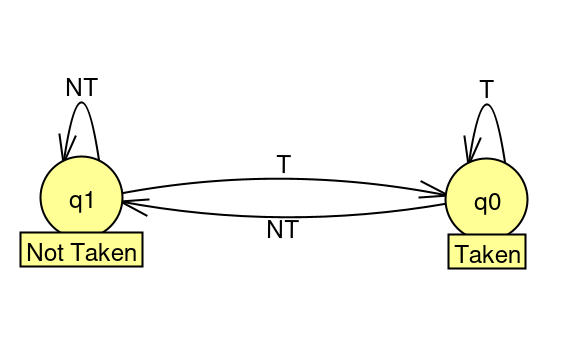
\includegraphics[scale=0.8]{preditor_de_1_bit}
                                            \caption{Maquina de estado finito que representa o preditor de 1 bit.}
                                        \end{figure}
                                        \item Ele tem problemas com loop alinhados pois ele vai acertar que o loop
                                            interno vai ser executado porém vai errar quando ele entrar de novo já que
                                            na hora que saiu ele erro e definiu NT só que na hora de entrar de novo ele
                                            erra e define como T.
                                    \end{itemize}
                                \item \textbf{PReditor de 2 bits}
                                    \begin{itemize}
                                        \item errar duas vezes a predição para mudar de estado (Taken/Not Taken).
                                            \begin{figure}
                                                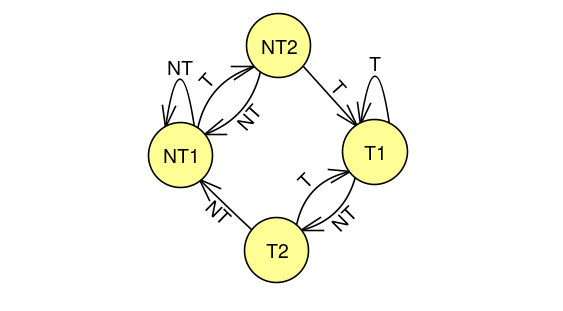
\includegraphics[scale=0.6]{imagens/preditor_de_2_bit.png}
                                                \caption{Maquina de estado finito que representa o preditor de 2 bit.}
                                            \end{figure}
                                    \end{itemize}
                                \item  \textbf{Desvios correlacionados}
                                    \begin{itemize}
                                        \item Decisão de tomada de decisão depende do desvio atual e dos desvios
                                            anteriores.
                                        \item Preditor de dois níveis  onde um bit preditor produz o que fazer se o
                                            desvio anterior foi tomado outro bit produz o que fazer se o desvio anterior
                                            não foi tomado.
                                    \end{itemize}
                            \end{itemize}
                        \item BTB(Branch Target Buffer) Salvar o endereço destino do branch além da predição. Faz com
                            que não tenha necessidade de calcular o endereço de novo.
\begin{table}
    \begin{center}
        \begin{tabular}{c|c|c}
            \textbf{PC} & \textbf{PC previsto} & \textbf{Predição}\\
            \hline
            Bit Menos Significativo & Endereço destino & T
        \end{tabular}
    \end{center}
\end{table}
                    \end{itemize}
            \end{itemize}
    \end{enumerate}

\section{Pipeline Avançado}
\subsection{Introdução}
No processador há níveis de paralelismo o nível mais básico é o BLP(Bit Level Parallelism) que é o monociclo, já que é
utilizado o fato de que é possível operar por todos os bits de um dado ao mesmo tempo.

Outro nível é o ILP (Instruction Level Paralellism) é o paralelismo entre instruções(Pipeline) pode ser feito de duas formas:
\begin{itemize}
    \item Aumentar o nível de produndidade do pipeline.
    \item Replicar os componentes da arquitetura de modo a iniciar mais de uma instrução em cada estágio do pipeline
        (\textbf{Despacho Mútiplo})
\end{itemize}

\subsection{Despacho de Instruções}
Despacho é o númeto de instruções disparadas ao mesmo tempo. Para isso é necessário replicar os componentes do
processador, por exemplo a necessidade de duas ULAs para que as duas instruções do estágio EX possam executar ao mesmo
tempo.

O despacho Mútiplo pode ser feito de forma estático ou Dinâmico.

\subsubsection{Despacho Mútiplo Estático}
    As decisões sobre quais instruções serão despachadas ao mesmo tempo é feita pelo compilador.

    É utilizado um pacote de despacho que é um conjunto de instruções, ou seja uma única instrução com varias operações
    chamada de VLIW(Very Long Instruction Word).

    \textbf{Coloca a imagem da instrução e a da arquitetura do MIPS}

    MIPS é feito utilizando uma VLIW de duas palavras, sendo que na primeira instrução tem que ser do tipo R, branch ou
    TipoI, enquanto no segundo slot é colocado as lw/sw. Para isso é necessário repliar as entradas do banco de
    registrador e a ULA. Nessa arquitetura o compilador cuida das dependências de dados e de controle.

    \textbf{Ex.:}

    Loop: lw \$t0, 0 (\$s1)
    addu \$t0,\$t0,\$s2
    sw \$t0 , 0 (\$s1)
    addi \$s1 , \$s1, -4
    bne \$s1 , \$zero , loop

\begin{table}[h]
    \begin{center}
        \begin{tabular}{||c|c|c||}
            \hline
            & \textbf{1º Instr} & \textbf{2º Instr}\\
            \hline
            Loop & & lw \$t0, 0 (\$s1)\\
                 & addi \$s1 , \$s1, -4 & \\
                 & addu \$t0,\$t0,\$s2 & \\
                 & bne \$s1 , \$zero , loop & sw \$t0 , 4 (\$s1)\\
            \hline

        \end{tabular}
    \end{center}
\end{table}

    Desdobramento de loop - Loop Unrolling é uma técnica usada pelo compilador para tentar aproveitar melor os slots do
    despacho múltiplo estático, ele basicamente faz em código mais de uma iteração do loop de uma vez, por exemplo o
    loop anterior pode ser feito em hardware 4 vezes.

\begin{table}[h]
    \begin{center}
        \begin{tabular}{||c|c|c||}
            \hline
            & \textbf{1º Instr} & \textbf{2º Instr}\\
            \hline
            Loop & addi, \$s1 , \$s1, -16 & lw \$t0, 0 (\$s1)\\
                 &                        & lw \$t1 , 12(\$s1)\\
                 & addu \$t0, \$t0, \$s2  & lw \$t2 , 8(\$s1)\\
                 & addu \$t1, \$t1, \$s2  & lw \$t3 , 4(\$s1)\\
                 & addu \$t2, \$t2, \$s2  & sw \$t0 , 16(\$s1)\\
                 & addu \$t3, \$t3, \$s2  & sw \$t1 , 12(\$s1)\\
                 &                        & sw \$t2 , 8(\$s1)\\
                 & bne \$s1 , \$zero , loop & sw \$t3 , 4(\$s1)\\
            \hline

        \end{tabular}
    \end{center}
\end{table}

\subsubsection{Despacho Mútiplo Dinâmico}
    As decisões sobre quais instruções serão despachadas ao mesmo tempo é feita pela arquitetura.\\
    Dessa forma o código objeto de uma arquitetura superescalar é igual ao de uma arquitetura convencional.\\
    É organizada como múltiplos pipelinesa ou seja tem dois IF,dois ID, dois EX,..etc\\
    Isso é fácil para os estados IF e ID, pois é só dobrar a unidade de busca de instrução e de decodificação.Já os
    estados MEM e WB é necessário aumenta ros canais de escrita na memória e banco de registradores. A Ex só necessita
    dublicar a ULA.\\
    Todas as arquiteturas modernas utilizam despacho múltiplo dinâmico.\\
    Faz muito sentido se você conseguir alterar a ondem das instruções, dessa forma conseguindo juntar mais instruções
    em uma mesma instrução.\\

\subsubsection{Conclusão}
    Para determinar se é estático (VLW) ou dinâmico é ver quem cuida do despacho o compilador(estático) ou a
    arquitetura.

\subsection{Escalonamento de Instrução}
    O escalonamento das instruções tem como base a especulação, ou seja o processador ou o compilador tentam advinhar o
    resultado de uma instrução para removê-la como dependência na execução das instruções.
\subsubsection{Escalonamento Estático} É feito pelo compilador.
\subsubsection{Escalonamento Dinâmico}
    A arquitetura escolhe quais instruções serão executadas em seguida , possivelmente reordenando para evitar parada.\\
    Para implementar a execução fora d eordem, tem-se que dividir o estágio de decodificação em 2.\\
    Despacho: decodifica a instrução e procura por hazards estruturais.\\
    ler os operandos esperar até que não tena hazard de dados, depois lê os operandos.\\
    Busca e decodificação in order.\\
    execução: out of order.\\
    Commit in order.\\

    Exemplo de escalonamento dinâmico:
    \begin{itemize}
        \item Scoreboard
        \item Tomasulo
    \end{itemize}


\subsection{Scoreboarding}
O scoreboard não é de despacho multiplo é uma forma de escalonamento dinâmico,
é feito com 3 tabelas:
\begin{itemize}
    \item Estado das instruções tem uma coluna para cada estágio.
        \begin{table}[h]
            \begin{center}
                \begin{tabular}{||c|c|c|c|c||}
                    \hline
                    Instrução&I&RO&EX&WR\\
                    \hline
                    X& o &o&&\\
                    \hline
                \end{tabular}
            \end{center}
        \end{table}
    \item Estado das unidades funcionais(UF) tem nove colunas
        \begin{enumerate}
            \item Busy
            \item Operação
            \item Fi = reg dst
            \item Fj = regOrigem
            \item Fk = regOrigem2
            \item Qj = UF que está produzindo o valor de Fj.
            \item Qk = UF que está produzindo o valor de Fk.
            \item Rj = flags que indicam que Fj esta pronto mas que não foi lido.
            \item Rk = flags que indicam que Fk esta pronto mas que não foi lido.
        \end{enumerate}
    \item Estado dos registradores de resultado. vai ter uma entrada para cada registrador disponível da
        arquitetura(F1,F2\ldots FN). marcando qual UF está produzindo um valor para o registrador.
\end{itemize}
Passos:
\begin{enumerate}
    \item Despacho(Issue). decodifica e verifica hazrd estrutural.
    \begin{itemize}
        \item \textbf{Condição de espera}(oq faz ele não deixar a instrução executar)
            \begin{itemize}
                \item UF(Unidade funcional) está  ocupada.
                \item uma outra instrução escreve no mesmo registrador de destino(WAW).
            \end{itemize}
        \item \textbf{Ações}(oq ele faz caso não tenha condição de espera)
            \begin{itemize}
                \item a instrução é enviada para a UF.
                \item o scoreboarding é  atualizado.
            \end{itemize}
    \end{itemize}
    \item Leitura dos operandos(Read Operands)
        \begin{itemize}
            \item \textbf{condição de espera}
                \begin{itemize}
                    \item Se Rj e Rk não estão prontos.
                \end{itemize}
            \item \textbf{Ações}
                \begin{itemize}
                    \item UF lê os operandos inicia a execução no proximo ciclo.
                \end{itemize}
        \end{itemize}
    \item Execução(Executor)
        \begin{itemize}
            \item \textbf{Ações}
                \begin{itemize}
                    \item a UF inicia a execução asism que recebe os dados
                    \item notifica o scoreboarding.
                \end{itemize}
        \end{itemize}
    \item Escrita dos resultados(Write result)
        \begin{itemize}
            \item  \textbf{Condição de espera}
                \begin{itemize}
                    \item Espera até que todos os resitradores operandos iguais ao registrador
                        destino sejam lidos.
                \end{itemize}
            \item \textbf{Ações}
                \begin{itemize}
                    \item escreve no registrador e atualiza o scoreboarding.
                \end{itemize}
        \end{itemize}

\end{enumerate}

\subsection{Tomasulo}
\textbf{Objetivo :} Foi feito para conseguir alto desempenho em operações de ponto flutuante.

A arquitetura tem pocuos registradores o que acarretou em mais problemas e depencência falsa ou de nome(WAW , WAR).

Soluções:
\begin{enumerate}
    \item Permitir que as operações iniciem a execução tão logo os operandos estiverem prontos(parecido com o
        forwarding)
    \item Implementar renomeação em hardware. (pois  a IBM queria aumentar a eficiência independente da arquitetura).
\end{enumerate}

Essa solução é implmentada utilizando 8 buffers distribuidos nas unidades funcionais e substituição dos registradores
nas instruções por valores ou apontadores para as estações de reserva(\textit{reservation stations} -RS) atráves de um
processo de renomeação de registradores, dess forma evita hazards(WAW ,WAR) e otimiza de forma melhor que o compilador
se existir mais estações de reserva que registradores.

Também é feito com 3 tabelas:
\begin{itemize}
    \item Register Result Status:
        \begin{itemize}
            \item funciona igual ao do scoreboard.
        \end{itemize}
    \item Instruction Status:
        \begin{itemize}
            \item funciona igual ao scoreboard
            \item só tem os membros, Issue , Execution Complete , Write Result
        \end{itemize}
    \item Reservation Station(RS)
        \begin{itemize}
            \item vai ser parecido com o do scoreboard e vai ter as seguintes colunas:
                \begin{itemize}
                    \item Busy -> indica se está em uso
                    \item Op   -> qual a operação.
                    \item $V_j$ e $V_k$ armazena o valor do registrador alvo.
                    \item $Q_jQ$ e $Q_k$ indica quem está produzindo o valor desejado.
                    \item A armazena o valor imediato, e o resultado da soma do imediato nas load/store.
                \end{itemize}
        \end{itemize}
\end{itemize}


\section{Curiosidades}
\subsection{Otimização de código}
    O compilador toma varias ações para tentar otimizar o código entre elas:
    \begin{itemize}
        \item Elimina expressões comuns.
        \item Elimina desvios desnecessários.
        \item Elimina código redundante.
        \item Altera a ordem de execução das instruções.
    \end{itemize}


\end{document}


